\chapter{What the crap is this?}
We will come back to this later. Bcoz we don't know what to write? 
\section{YYY??}
\subsection{Compare: one of the first mistaken attitudes!}
A typical transaction system lives inside the range of some gigabytes data, in random access. It runs inside an application server, acceses and takes control over a relational database allocated in a different server, transporting data in and out of it.
Interacts with online clients, keeping a reduced size of data in transport, with a shared and limited bandwith, the operations are most of all continuous reading over small sets of data, combined with some maintenance \& CRUD operations.
Bigger data processing is done in batch, but the architecture is the same.

\subsection{But a different scenario ?}
What happens if we need to process 1 petabyte/week ?, let's say a much lesser size, 1 terabyte/day, less, 100 gigabytes/day
Under the traditional schema, it would be like moving an elephant over a string thousands of times, the time-windows would not allow to work with realtime information, but always trying to keep up and losing the race.

\subsection{Want problems ?}
The network would saturate, batch processes would take days to finish information of hours, the harddisk latency access it will transform into an incremental overhead, having a painful impact on overall costs.
The traditional approach would mantain the architecture, but changing hardware, sophisticated requirements, each time more expensive, bigger, but over a limited growth architecture. How many times will you change your system's architecture to non-linear scalar solutions to keep up with the race of growing data, ?

\subsection{The solution is in the focus !}
\textcolor{red} {Problem 1: Size of data} \\
Systems handling public data, can have huge processing flows with hundreds of terabytes, public websites have had increased their data up to petabytes ! \\
\textcolor{blue} {Strategy 1: Distribute and paralellize the processing} \\
If chewing 200 Tb of data takes 11 days in 1 computer, let divide the whole process into as many machines needed to finish the task in minutes or hours !
If we'll have lot of computers, so be they cheap and easily mantained !, into a simple add \& replace node architecture.

\textcolor{red} {Problem 2: Continuous failure and cluster growth} \\
In a big cluster, lot of machines fail everyday, besides the cluster size cannot be fixed and sometimes cannot be planned, it should grow easily at the speed of data. \\
\textcolor{blue} {Strategy 2: High fault tolerance and high scalability} \\
Any design must have an excelent fault-tolerance mechanism, a very flexible maintenance, and its service availability should keep up naturally to its cluster size.
So we need a distributed storage, atomic, transactional, with perfect linear scalability. \\

\textcolor{red} {Problem 3: Exponential overhead in data transport} \\
From data source to its processing location, bad harddisk latency and saturated networks will end up exploting \\
\textcolor{blue} {Strategy 3: Move application logic to data storage}
It must allow to handle data and processes separately and in a transparent way, applications should take care of their own business application code, and the platform should automatically deploy it into the datastorage, execute and handle their results, 

So...
Distribute and Paralellize processing
High fault-tolerance mechanism, High scalability
Take application processes to data storage

One Solution: Hadoop Distributed Filesystem + Hadoop MapReduce

Anyway, Hadoop is not bullet-proof, actually, it's a very specific solution for some big-data scenarios, with needs of realtime processing, and technology choices for random access to data. (See HBase, Hive)

Hadoop is not designed to replace RDBMS, but instead, has been proven to handle -in a much performant way- huge amounts of data, whereas traditional enterprise database clusters, wouldn't work not even close at the same overall costs !

\chapter{Architecture}

\section{FileSystem}
\begin{itemize}
\item Scales linearly over a set of low-budget comodity machines, doubled the amount of machines = reduced the processing time to half
\item Tolerates faults at different levels, from network, switches, disks, nodes, readdressing data traffic to other nodes, accomplishing a replica factor
\item Flexible scalability, for maintenance tasks, you only have to dis/connect computers into the rack
\item Lets you allocate any kind of files and formats, although it has better performance on files bigger than 128mb
\item The results of MapReduce jobs are stored in the filesystem
\item There's a unique namespace, with an automatic replication schema administered by the master, it's not possible to impact on a certain node in the cluster, whether to allocate files or execute jobs
\item The master itself balances the workload over execution plans and status reports from the slave nodes
\item Has a mechanism of continuous replication per file, rack-aware, to extend data reliability and data availability warranties
\item Has an automatic file checksum with inmediate correction
\item Works in a master-slave schema where slaves share nothing between them, they only respond to master requests
\item The master coordinates all types of transactions, read/write, replication, restore, manages the tx log and the filesystem namespace
\item The slaves only take charge on low level operations over data, read, write, deletion, transport to-from client
\end{itemize}

\begin{figure}
\caption{The picture shows a more practical brief over HDFS responsibilities \& execution flows}
\label{tab:hdfs_resposibilities_and_execution_flow}
\centering
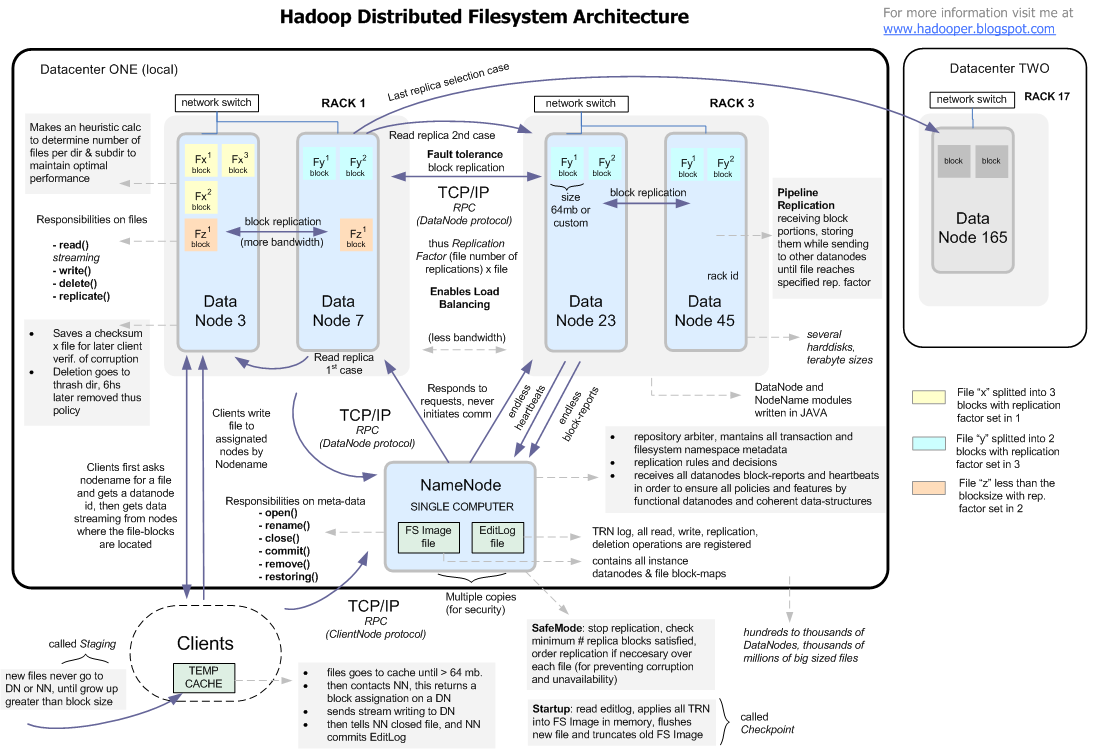
\includegraphics[scale=.33]{./img/HadoopDFSArchitecture.png}
\end{figure}


\section{Processing Model}
Main characteristics of Map Reduce   \\

\begin{itemize}
\item It's a processing model about dividing and distributing information, in two chained phases: map first, then reduce
\item Both phases have as input and output, a key-value pair list, 
\item The schema allows to define method parameters and own logic for both phases, as well as their own partitioning system and intermediate storage between phases.
\item The transactions are handled by a JobTracker daemon, that runs the initial data partitioning and the intermediate data combination, by posting tasks of type Map and type Reduce over the TaskTracker daemons (1-n x computer) of the nodes involved in the cluster, according the data being processed
\item The Reduce phase only starts when finished the Map, cause after the Map the resulting keys are combined, to distribute a sorted list of key-value pairs between the Reducers, that can be matched at the end of them.
\item The process is transactional, those map or reduce tasks not executed, (for data availability issues) will be reattempted a number of times, and then redistributed to other nodes.
\end{itemize}

\begin{figure}
\caption{The picture shows how these methods will interact in phases.}
\label{tab:hadoop_map_reduce_cycle}
\centering
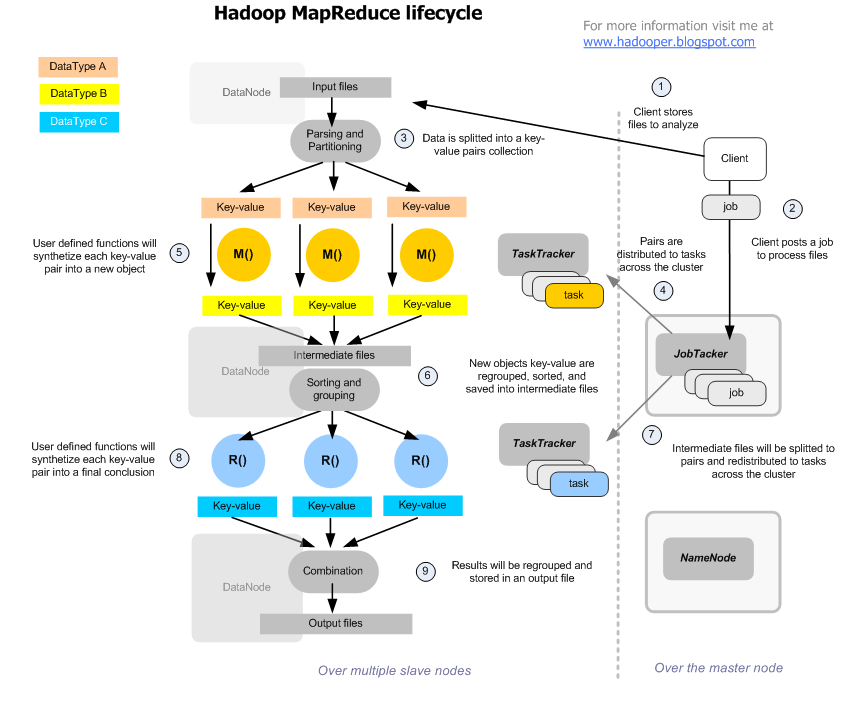
\includegraphics[scale=.33]{./img/HadoopMapReduceArchitecture.png}
\end{figure}

\begin{itemize}
\item First the files are partitioned in parts that will be distributed to process across the cluster nodes
\item  Each part is parsed in pairs of Key(sorteable object) - Value(object), that will be the input parameters for the tasks implementing the Map function
\item  These user defined tasks (map), will read the value object, do something with it, and then build a new key-value list that will be stored by the framework, in intermediate files.
\item  Once all the map tasks are finished, it means that the whole data to process was completely read, and reordered into this mapreduce model of key-value paris.
\item  These intermediate key-value results are combined, resulting a new paris of key-value that will be the input for the next reduce tasks
\item  These user defined tasks (reduce), will read the value object, do something with it, and then produce the 3rd and last list of key-value pairs, that the framework will combine, and regroup into a final result.

\end{itemize}
\begin{figure}
\caption{Let's see a sample job with a reverted-index function, for analyzing the webcrawler's output files (just for instance)}
\label{tab:hadoop_map_reduce_architecture}
\centering
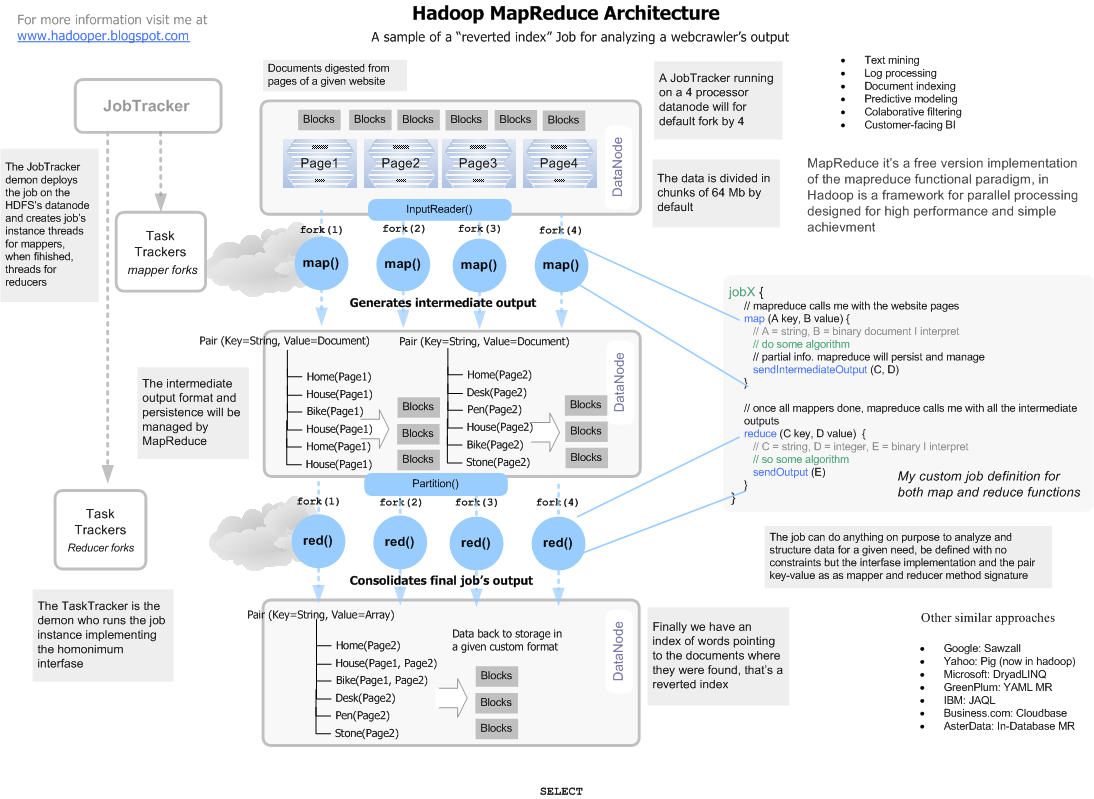
\includegraphics[scale=.33]{./img/HadoopMRProcessSample.png}
\end{figure}

MapReduce something, is about iterate a huge record collection, extract something good, mix and regroup intermediate results, that's all, it may look more complex than what it is.
